\documentclass[output=paper,modfonts]{langscibook}
\title{A transition-based verbal multiword expression analyzer} 
\author{Hazem Al Saied\affiliation{ATILF UMR 7118, Universit\'e de Lorraine/CNRS}\and  Marie Candito\affiliation{LLF UMR 7110, Universit\'e Paris Diderot/CNRS}\lastand   Matthieu Constant\affiliation{ATILF UMR 7118, Universit\'e de Lorraine/CNRS}}
\abstract{ We describe a robust transition-based analyzer for identifying and categorizing Verbal Multiword Expressions (VMWEs). The system was developed and evaluated using the datasets of the PARSEME shared task on VMWE identification \citep{MWEWorkshop}.\newline We accommodate the variety of linguistic resources provided for each language, in terms of accompanying morphological and syntactic information. Our system produces very competitive scores, for both VMWE identification and categorization, with respect to the shared task results.}
\begin{document}
\maketitle
\label{ALSAIED-CHAPTER}
% ***********************************
%			Introduction
% ***********************************
\section{Introduction}
We present a generic system for the identification and categorization\is{verbal multiword expression!identification}\is{verbal multiword expression!categorization} of verbal multiword expressions (hereafter VMWEs).
With respect to grammatical or nominal multiword expressions, VMWEs tend to exhibit more morphological and syntactic variation than other MWEs, if only because in general the verb is inflected and can receive adverbial modifiers. Furthermore, some VMWE types, in particular light-verb constructions, allow for the full range of syntactic variation (extraction, coordination etc...). This renders the VMWE identification task even more challenging than general MWE identification, in which fully frozen and continuous expressions contribute to an increase in the overall performance.

Our objective was to design a data-driven system applicable to several languages, with limited language-specific tuning. We took advantage of the datasets provided within the shared task\is{PARSEME!shared task} on automatic identification of VMWEs \citep{MWEWorkshop} to train and test our system.
These datasets concern 18 languages, and consist of tokenized sentences in which VMWEs are annotated. One VMWE instance is a set made either of several tokens, potentially non-continuous, or of one single token  (i.e. a multiword token, hereafter MWT, such as amalgamated verb-particle in \ili{German}).\footnote{The majority of annotated VMWEs are multi-token. The prevalence of MWTs varies greatly among languages. While absent from seven languages and very rare for nine other languages, they are very frequent in \ili{German} and \ili{Hungarian}.} A VMWE may be embedded in another longer one, and two VMWEs can overlap. Each annotated VMWE is tagged with a category among Light-Verb Constructions (LVC), IDioms (ID), Inherently REFLexive Verbs (IReflV), Verb-Particle Constructions (VPC) and OTHer verbal MWEs (OTH). The datasets are quite heterogeneous, both in terms of size and of accompanying resources: 4 languages have none (\ili{Bulgarian}, \ili{Spanish}, \ili{Hebrew}, \ili{Lithuanian}), for 4 languages, morphological information such as lemmas and POS is provided (\ili{Czech}, \ili{Maltese}, \ili{Romanian}, Slovene), and for the 10 remaining languages, full dependency parses are provided.

The system we describe in the current paper is an extension of the ATILF-LLF system \citep{W17-1717}, a one-pass greedy transition-based\is{parsing!transition-based} system which participated in the shared task\is{PARSEME!shared task}, obtaining very competitive results (hereafter ATILF-LLF 1). The new system (ATILF-LLF 2) categorizes the VMWEs on top of identifying them, and has an extended expressive power, handling some cases of VMWE embedded in another one. Both for ATILF-LLF 1 and 2, we tuned a set of feature template\is{feature!template} for each language, relying exclusively on training data, accompanying CoNLL-U files when available, and basic feature engineering.

The remainder of the article is organized as follows: we describe our system in Section 2, and comment its expressive power as opposed to ATILF-LLF 1. We then describe the experimental setup in Section 3, and comment the results in Section 4. Section 5 is devoted to related work. We conclude in Section 6 and give perspectives for future work. 

% *********************************** 
%			System description
% ***********************************
\section{System description}

The analyzers we developed (ATILF-LLF 1 and 2) are simplified versions of the system proposed by \citet{constant-nivre:acl:2016}. Building on the classic arc-standard dependency parser \citep{nivre04acl}, \citet{constant-nivre:acl:2016} designed a parsing algorithm that jointly predicts a syntactic dependency tree and a forest of multiword lexical units\is{parsing!dependency}. Their system uses both a syntactic and a lexical stack and specific transitions merge tokens to create MWEs, as proposed by \citet{Nivre14}. We have simplified this formal apparatus keeping only the lexical stack, and predicting MWEs only.

A transition-based\is{parsing!transition-based} system applies a sequence of actions (usually called \emph{transitions}) to incrementally build the expected output structure in a bottom-up manner. Each transition is usually predicted by a classifier given the current state of the system (namely a \emph{configuration}).

A configuration in our system consists of a triplet $c = (\sigma, \beta, L)$, where $\sigma$ is a stack containing units under processing, $\beta$ is a buffer containing the remaining input tokens, and $L$ is a set of output MWEs.

The \emph{initial configuration} for a sentence $x = x_1, ..., x_n$, i.e. a sequence of $n$ tokens, is represented by $c_s$ as: $c_s (x) = ([], [x_1, \ldots, x_n], \emptyset)$ and the set of \emph{terminal configurations} $C_t$ contains any configuration of the form $c_t = ([], [], L)$. At the end of the analysis, the identified VMWEs are simply extracted from $L$.

Single tokens are brought to the stack by the \textsc{Shift} transition, and are potentially marked as (mono-token) VMWE using the \textsc{Mark as C} transition, whereas trees are formed using merge transitions (cf.  \sectref{sec:transitionset}).

The output VMWEs are the units added to $L$, either by the \textsc{Mark as C} or \textsc{Merge as C} transitions. When one VMWE is embedded in another one, both VMWEs appear separately in $L$ (which is thus redundant).\footnote{For instance, if we represent the binary tree in bracketing format and the categorization with a subscript, $( (a, b)_{IReflV}, c )_{ID}$ represents an IReflV $a+b$ embedded within an ID $a+b+c$. Both $( (a, b)_{IReflV}, c )_{ID}$ and $(a, b)_{IReflV}$ will appear in $L$.}

% ***********************************
%			Transition set
% ***********************************
\subsection{Transition set} 
\label{sec:transitionset}

Our system uses the following transitions: 
\begin{enumerate}
\item the \textsc{\textbf{Shift}} transition moves the first element of the buffer to the stack
\begin{itemize}
\item[] \textbf{Precondition}: the buffer is not empty.
\end{itemize}
\largerpage
\item the \textsc{\textbf{Reduce}} removes the top element of the stack
\begin{itemize}
\item[] \textbf{Precondition}: the stack is not empty.
\end{itemize}
\item the \textbf{\textsc{White Merge}} transition combines the two top elements of the stack into a single element;  
\begin{itemize}
\item[] \textbf{Precondition}: the stack contains at least two elements.
\end{itemize}
\item five \textsc{\textbf{Merge As \textbf{C}}} transitions (where \textbf{C} stands for a VMWE category) perform a white merge, mark the resulting unit as a VMWE of category \textsc{C}, and add it to $L$.
\begin{itemize}
\item[] \textbf{Precondition}: the stack contains at least two elements.
\end{itemize}
\item In order to cope with MWTs, we added five \textsc{\textbf{Mark as \emph{C}}} transitions, which mark the top stack element as a VMWE, assign to it the category \textsc{C}, and add it to $L$.
\begin{itemize}
\item[] \textbf{Precondition}: The stack is not empty and its head is a non-marked single token.\footnote{Because mono- and multi-tokens have very different linguistic properties, we preferred to distinguish transitions coping with both kinds of VMWEs. Without this restriction, as noted by a reviewer, \textsc{Merge as C} would be equivalent to \textsc{White Merge + Mark as C}. The effectiveness of this alternative solution remains to be tested.}
\end{itemize}
\end{enumerate}
\figref{ex:parse} shows the analysis of a \ili{German} sentence containing a \isi{multiword token} VPC embedded within an IReflV.
% ***********************************
%			Figure ex:parse
% ***********************************
\begin{figure}[h]
\footnotesize
\centering
\fbox{
\begin{tabular}{lll}
\\[-0.2cm]
\textbf{Transition} & & \textbf{Configuration} \\
& & $~[~], [\mbox{Damit}, \mbox{müsste},\mbox{man}, \mbox{sich}, \mbox{nun}, \mbox{herumschlagen}], [~]~$\\
Shift&$\Rightarrow$& $~[\mbox{Damit}], [\mbox{müsste}, \mbox{man}, \mbox{sich}, \mbox{nun}, \mbox{herumschlagen}], [~]~$\\
Reduce&$\Rightarrow$& $~[~], [\mbox{müsste}, \mbox{man}, \mbox{sich}, \mbox{nun}, \mbox{herumschlagen}], [~]~$\\
Shift&$\Rightarrow$& $~[\mbox{müsste}], [\mbox{man}, \mbox{sich}, \mbox{nun}, \mbox{herumschlagen}], [~]~$\\
Reduce&$\Rightarrow$& $~[~], [\mbox{man}, \mbox{sich}, \mbox{nun}, \mbox{herumschlagen}], [~]~$\\
Shift&$\Rightarrow$& $~[\mbox{man}], [\mbox{sich}, \mbox{nun}, \mbox{herumschlagen}], [~]~$\\
Reduce&$\Rightarrow$& $~[~], [\mbox{sich}, \mbox{nun}, \mbox{herumschlagen}], [~]~$\\
Shift&$\Rightarrow$& $~[\mbox{sich}], [\mbox{nun}, \mbox{herumschlagen}], [~]~$\\
Shift&$\Rightarrow$& $~[\mbox{sich}, \mbox{nun}], [\mbox{herumschlagen}], [~]~$\\
Reduce&$\Rightarrow$& $~[\mbox{sich} ], [\mbox{herumschlagen}], [~]~$\\
Shift&$\Rightarrow$& $~[\mbox{sich}, \mbox{herumschlagen}], [~], [~]~$\\
Mark as VPC&$\Rightarrow$& $[\mbox{sich},\mbox{herumschlagen}_{VPC}], [~], [\mbox{herumschlagen}_{VPC}]~$\\
Merge as IreflV&$\Rightarrow$& $~[(\mbox{sich},\mbox{herumschlagen}_{VPC})_{IReflV}], [~], $\\
               &            &  $~~ [\mbox{herumschlagen}_{VPC}, (\mbox{sich},\mbox{herumschlagen}_{VPC})_{IReflV}]~$\\
Reduce&$\Rightarrow$& $~[~], [~], [\mbox{herumschlagen}_{VPC}, (\mbox{sich},\mbox{herumschlagen}_{VPC})_{IReflV}]~$\\
\end{tabular}
}
\caption{Transition sequence for tagging the German sentence \exlitidio{Damit müsste man \lex{sich} nun \lex{herumschlagen}}{With-that must-SUBJUNCTIVE one REFLEXIVE now around-struggle}{One would have to struggle with that}
%\textsc{ Damit müsste man \textbf{sich} nun \textbf{herumschlagen}
%(With-that must-SUBJUNCTIVE one REFLEXIVE now around-struggle}, lit). \textit{'One would have to struggle with that'}
, containing two VMWEs: \textsc{sich herumschlagen} tagged as inherently reflexive verb (IReflV), in which \textsc{herumschlagen} is itself a multiword token tagged as verb-particle combination (VPC). 
}
\label{ex:parse}
\end{figure} 

In the input, each token is associated with linguistic attributes (form, and depending on the data sets, lemma and POS). When a merge transition is applied, the newly created element gets its attributes using basic concatenation over forms, and over lemmas and POS tags when available.\footnote{This would deserve to be improved in future experiments, with finer procedures to predict the lemmatized form and more importantly to predict the POS tag of the merged node, although in the special case of VMWE prediction the POS is verbal.}
% ***********************************
%			Parsing algorithm and training oracle
% ***********************************
\subsection{Parsing algorithm and training oracle}
\largerpage
In all the following, at parsing\is{parsing!transition-based} time we use a greedy algorithm, starting with an initial configuration $c_s$, and applying in sequence the best-scoring legal transition until a terminal configuration is reached.\footnote{Sentence analysis is composed of exactly $2n + r$ transitions, with $n$ being the number of tokens and $r$ the number of MWTs. Every single token not entering a VMWE requires a \textsc{Shift} and a \textsc{Reduce}, every multi-token VMWE of length $m$ requires $2m$ transitions ($m$ \textsc{Shifts}, $m-2$ \textsc{White Merges}, one \textsc{Merge As C} and one \textsc{Reduce}), while every MWT requires three transitions: a \textsc{Shift}, a \textsc{Mark As C} and a \textsc{Reduce}.}

The training phase learns the transition-scoring classifier. This is done through supervised learning, by converting the training sentences into sequences of [configuration, gold transition to apply] pairs, by using a static oracle.\footnote{Using \citep{goldberg2013training}'s terminology, a static oracle is both incomplete (defined for configurations obtained from previous oracle transitions only) and deterministic (at each such configuration, there is a single oracle transition to apply).} Our static oracle returns for a given configuration the first applicable transition using the following priority order: \textsc{Mark as C, Merge As C, White Merge, Reduce} and \textsc{Shift}. Applicability here means not only the standard preconditions for transitions, but also that the output configuration is compatible with the gold annotations. We added the constraint that the {\textsc{White Merge}} is only applicable to the right suffix of a gold VMWE. For instance, suppose we have a gold continuous VMWE \textit{kick the bucket}, when the first two elements are on top of the stack, the \textsc{White Merge} is not applicable yet, it will be applied when the right suffix \textit{the} and \textit{bucket} is on top of the stack.

To produce our training examples, we start by generating the initial configuration for each sentence, and apply in sequence the transition predicted by the static oracle, until a terminal configuration is reached. 
The analysis in \figref{ex:parse} corresponds to the oracle transition sequence for the example sentence.
% ***********************************
%			Expressive power
% ***********************************
\subsection{Expressive power}
As far as expressive power is concerned, ATILF-LLF 2 is slightly more powerful than ATILF-LLF 1. ATILF-LLF 2 now performs VMWE categorization\is{verbal multiword expression!categorization} and not just identification. Both systems cannot analyze interleaving MWEs, but while ATILF-LLF 1 could cope with no overlapping\is{verbal multiword expression!overlapping} at all, ATILF-LLF 2 can cope with some cases of embeddings, i.e. some cases of VMWE fully contained in another one.\footnote{It is worth noting that embedded VMWEs are very rare in the datasets: there are twenty to thirty embedded VMWEs in German, Hebrew and Hungarian and about 150 in Czech.}

In effect, ATILF-LLF 1 contained a \textsc{Shift} transition, a \textsc{White merge}, a \textsc{Merge as C+Reduce} for identifying multi-token VMWEs, and a \textsc{Mark as C+Reduce} for MWTs.\footnote{ATILF-LLF 1 used hard-coded procedures for matching MWTs (if seen in the training set), which we replaced by features used by the classifier.} Because the \textsc{Merge as C+Reduce} transition identifies a MWE and removes it from the stack, no cases of embeddings were covered.

In ATILF-LLF 2, some cases of embeddings are now covered (e.g. the example in \figref{ex:parse}). More precisely, the covered cases are those where one can form a projective tree by attaching to a fictitious root all the binary trees representing the VMWEs of a sentence, ignoring tokens not belonging to any VMWE. An alternative formulation is that given any VMWE composed of the $t_1 t_2 ... t_m$ tokens and any gap $g_1 g_2 ... g_n$ appearing between a pair of components $t_i t_{i+1}$, the condition is that the $g_i$ tokens cannot belong to a MWE having components outside the set $g_1 ... g_n$. So a non-covered case is found for instance in \textsc{\textbf{{Let$_{1,2}$}} {the$_{1}$} {cat$_{1}$} \textbf{{out$_{1,2}$}} {of$_{1}$} {the$_{1}$}  {bag$_{1}$}}: the VMWE \textsc{\textbf{Let out}} has a gap containing tokens \textsc{{the$_{1}$} {cat$_{1}$}}, which belong to a VMWE with tokens outside the gap.

% ***********************************
%			Experimental setup
% ***********************************
\section{Experimental setup}
For a given language, and a given train/dev split, we use the oracle-based resulting transition sequences to train a multi-class SVM classifier\is{support vector machine}.\footnote{The whole system was developed using Python 2.7, with 4,739 lines of code, using the Scikit-learn 0.19. We used the Error-correcting output codes framework for the multi-class SVM classifier. The code is available on Github: \url{https://goo.gl/1j8mVu} under the MIT license.}
We describe in the next subsections the feature templates we used (\sectref{ss:features}) and how we tuned them (\sectref{ss:tuning}). 
% ***********************************
%			Table
% ***********************************

\begin{table}[t]
\centering
\small
\begin{tabular}{ll}
\lsptoprule
\textbf{Code}&\textbf{Setting description}\\
\midrule
A &use of POS and lemmas\\
A' & use of suffixes\\
B &use of syntactic dependencies\\
C &use of bigrams S$_1$S$_0$, S$_0$B$_0$, S$_1$B$_0$ and S$_0$B$_1$\\
D &use of the trigram S$_1$S$_0$B$_0$ \\
E &use of the S$_0$B$_2$ bigram\\
F &use of transition history (length 1)\\
G &use of transition history (length 2)\\
H &use of transition history (length 3)\\
I &use of distance between S$_0$ and S$_1$\\
J &use of distance between S$_0$ and B$_0$\\
K &use of B$_1$\\
L &use of training corpus VMWE lexicon\\
M &use of stack length\\
N &use of MWT dictionary\\
\lspbottomrule
\end{tabular}
\caption{System setting code descriptions.}
\label{table:codes}
\end{table}
% ***********************************
%			Feature Templates
% ***********************************
\subsection{Feature templates}
\label{ss:features}
A key point in a classical transition-based system\is{parsing!transition-based} is feature engineering, known to have great impact on performance. 
We have gathered feature templates\is{feature!template} into groups, for which we provide short descriptions in \tabref{table:codes}, along with code letters that we use in \sectref{sec:results} to describe which feature groups were used for each language in the final shared task results. We describe in this section each feature group. We hereafter use symbol $B_i$ to indicate the $\textsc{i}$th element in the buffer. $S_0$ and $S_1$ stand for the top and the second elements of the stack. For every unit $X$ in the stack or buffer, we denote $X_w$ its word form, $X_l$ its lemma and $X_p$ its POS tag. The concatenation of two elements $X$ and $Y$ is noted $XY$. 
% ***********************************
%			Basic Linguistic Features
% ***********************************
\subsubsection*{Basic linguistic features}
\largerpage[-1]
For each language, we used a precise set of stack or buffer elements, hereafter the {\em focused elements}, to derive unigram, bigram and trigram features. By default, the focused elements are $S_0$, $S_1$ and $B_0$. For some languages, $B_1$ was also used (code K in \tabref{table:codes}). If bigrams are on (code C in \tabref{table:codes}) features are generated for the element pairs $S_1 S_0$, $S_0B_0$, $S_1B_0$, plus $S_0B_1$ if K is on, and plus $S_0B_2$ for a few languages (code E). For trigrams, we only used the features of the $S_1S_0B_0$ triple (code D).

For any resulting unigram, bigram or trigram, we use by default the word form (e.g. $S_{0w}$). For languages whose datasets comprise morphological information, we further use the lemmas and POS tags (code A in \tabref{table:codes}), i.e. $X_l$ and $X_p$. The precise features for a bigram $XY$ are $X_wY_w$, $X_pY_p$, $X_lY_l$, $X_pY_l$ and $X_lY_p$. Those for a trigram $XYZ$ are $X_wY_wZ_w$, $X_lY_lZ_l$, $X_pY_pZ_p$, $X_lY_pZ_p$, $X_pY_lZ_p$, $X_pY_pZ_l$, $X_lY_lZ_p$, $X_lY_pZ_l$, $X_pY_lZ_l$.

For the languages lacking companion morphological information, we tried to mimic that information using suffixes (code A' in \tabref{table:codes}), more precisely the last two and last three letters, which we used for unigram elements only.
% ***********************************
%			Syntax-based Features
% ***********************************
\subsubsection*{Syntax-based features}
After integrating classical linguistic attributes, we investigated using more linguistically sophisticated features. First of all, syntactic structure is known to help MWE identification\is{verbal multiword expression!identification} \citep{fazly-cook-stevenson:2009:CL,seretan2011syntax,nagyt-vincze:2014:MWE}. So for datasets comprising syntactic information, we introduced features capturing the existence of syntactic dependencies between elements of the buffer and of the stack (code B in \tabref{table:codes}).  More precisely, provided that $S_0$ is a single token, we generate (i) the features \textbf{\textsc{RightDep (S$_0$, B$_i$) = True}} and \textbf{\textsc{RightDepLab (S$_0$, B$_i$) = l}} for each buffer token B$_i$ that is a syntactic dependent of $S_0$ with label $l$, and (ii) the features \textbf{\textsc{LeftDep (S$_0$, B$_i$) = True}} and \textbf{\textsc{LeftDepLab (S$_0$, B$_i$) = l}} when a buffer element $B_i$ is $S_0$'s syntactic governor.

Other syntax-based features aim at modeling the direction and label of a syntactic relation between the top two tokens of the stack (feature \textbf{\textsc{syntacticRelation (S$_0$, S$_1$) = $\pm$ l }} is used for S$_0$ governing/governed by S$_1$, provided $S_0$ and $S_1$ are single tokens).\footnote{For ATILF-LLF 1, we used gold syntactic features for the languages accompanied with gold dependency companion files, as authorized in the closed track. Performance when using predicted syntax will be evaluated in future work.} All these syntactic features try to capture syntactic regularities between the tokens composing a VMWE.
% ***********************************
%			Misc. Features
% ***********************************
\subsubsection*{Miscellaneous features}
We found that other traditional features, used in transition-based\is{parsing!transition-based} systems,  were sometimes useful like  (local) transition history of the system. We thus added \textbf{History-based features} to represent the sequence of previous transitions (of length one, two or three, cf. codes F, G and H \-in  \tabref{table:codes}).

We also added \textbf{Distance-based features}, known to help transition-based dependency parsing\is{parsing!transition-based} \citep{zhang2011transition}, more precisely the distance between S$_0$ and  S$_1$ and between S$_0$ and B$_0$ (respectively codes I and J in \tabref{table:codes}). We also extracted \textbf{Stack-length-based features} (code M in  \tabref{table:codes}).

The VMWE identification\is{verbal multiword expression!identification} task is highly lexical so we found it useful to use \textbf{dictionary-based features}, which use ``dictionaries" extracted from the training set, both for multi-token VMWEs and MWTs. The dictionaries are lemma-based when lemmas are available, and form-based otherwise. These dictionary-based features include (i) a boolean feature set to true when S$_0$ belongs to the MWT dictionary (code N in  \tabref{table:codes}), and (ii) boolean features firing when $S_0$, $S_1$, $B_0$, $B_1$ or $B_2$ belong to an entry of the extracted VMWE dictionary (code L in \tabref{table:codes}).
% ***********************************
%			Feature Tuning
% ***********************************
\subsection{Feature tuning}
\label{ss:tuning}
We first divided the data sets into three groups, based on the availability of CoNLL-U files: (a) for \textbf{\ili{Bulgarian}, \ili{Hebrew}} and \textbf{\ili{Lithuanian}} neither morphological nor syntactic information is available on top of tokens and VMWE annotation; (b) \textbf{\ili{Czech}, \ili{Spanish}, \ili{Farsi}, \ili{Maltese}} and \textbf{\ili{Romanian}} are accompanied by CoNLL-U files with morphological information only, and (c) \textbf{the other languages}\footnote{These languages are German, Greek, French, Hungarian, Italian, Polish, Portuguese, Slovene, Swedish, and Turkish.} 
are accompanied by a fully annotated CoNLL-U file. 

In the first tuning phase, we used one ``pilot" language for each group (\ili{Bulgarian}, \ili{Czech} and \ili{French}). Then, \ili{German} was added as pilot language to investigate features for languages with high percentage of MWTs and embedded VMWEs. We tuned the features using both development sets extracted from the provided training sets, and using cross-validation.

Finally, we used the discovered feature groups as a source of inspiration for producing specialized feature groups for all other languages. Note that given the combinatorial explosion of feature combinations, we could not apply a full grid-search for the pilot languages, and a fortiori for all languages.
% ***********************************
%			Results
% ***********************************
\section{Results}
\label{sec:results}
% ***********************************
%			Table
% ***********************************
\begin{table}
 
\setlength\tabcolsep{4pt}
\fittable{
\begin{tabular}{lrrrrrrrrrl}
\lsptoprule
\multirow{3}{*}{} &  \multicolumn{6}{c}{Test dataset }  &\multicolumn{3}{c}{Cross validation }  &  \\ \cmidrule{2-10}
& \multicolumn{3}{c}{ VMWE-based F$_1$} & \multicolumn{3}{c}{Token-based F$_1$}& \multicolumn{3}{c}{VMWE-based F$_1$} & \\ \cmidrule{2-10}
\rot{Language}  & \rot{Baseline} & \rot{ATILF-LLF 2} & \rot{Best of ST} &\rot{Baseline} & \rot{ATILF-LLF 2}& \rot{Best of ST} & \rot{Baseline} &  \rot{ATILF-LLF 1} & \rot{ATILF-LLF 2} & Feature Settings  \\ 
\midrule
BG$^{**}$ 	& 47.6 			& 55.8 			& \textbf{61.3} & 50.7 & 60.2 & \textbf{66.2} & 48.3 & \textbf{57.1} & 53.0 & \scriptsize{A' C D F G I L } \\
CS$^*$ 	& 61.6 			& 70.9 			& \textbf{71.7} & 66.7 & \textbf{73.9} & 73.7 & 60.1 & \textbf{71.4} & 68.9 & \scriptsize{A C F G H I J K L M} \\
DE 	& 37.9 			& \textbf{45.8} & 41,1 & 33.3 & 44.8 & \textbf{*45.5} & 39.9 & 27.9 & \textbf{47.6} & \scriptsize{A B C D E J L N} \\
EL 	& 35.6 			& \textbf{42.8} & 40.1 & 39.9 & 46.3 & \textbf{46.9} & 48.0 & 56.2 & \textbf{57.3} & \scriptsize{A B C E J K L} \\
ES$^*$ 	& 56.9 			& \textbf{58.9} & 57.4 & 56.7 & \textbf{60.3} & 58.4 & 61.2 & 63.5 & \textbf{66.0} & \scriptsize{A C D F G H I J K L} \\
FA$^*$ 	& 72.2 			& 84.3 			& \textbf{86.6} & 72.5 & 84.8 & \textbf{90.2} & 67.3 & \textbf{87.7} & 81.1 & \scriptsize{A C I J K} \\
FR 	& 44.6 			& \textbf{60.6} & 57.7 & 49.3 & \textbf{62.6} & *61.5 & 66.0 & 71.1 & \textbf{73.8} & \scriptsize{A B C E I J K L} \\
HE$^{**}$ 	& \textbf{33.4} & 29.9 			& \textbf{33.4} & 29.6 & 30.5 & \textbf{31.3} & \textbf{30.0} & 17.0 & 26.8 & \scriptsize{A' C E F G H K L} \\
HU 	& 68.3 			& \textbf{74.8} & *74.0 & 64.9 & \textbf{72.1} & *70.8 & 73.7 & 23.5 & \textbf{83.7} & \scriptsize{A B C D F G H K L N} \\
IT 	& 39.2 			& 28.2 			& \textbf{39,9} & 39.5 & 29.8 & \textbf{43.6} & \textbf{33.7} & 27.4 & 27.2 & \scriptsize{A B C H J L} \\
LT$^{**}$ 	& 30.5 			& \textbf{34.1} & 28.4 & 27.3 & \textbf{31.7} & 25.3 & 20.7 & 8.6 & \textbf{21.5} & \scriptsize{A' C D E F G H I J K L M} \\
MT$^{*}$ 	& 8.2 			& 6.9 			& \textbf{14.4} & 12.3 & 9.4 & \textbf{16.3} & 7.7 & \textbf{8.1} & 7.2 & \scriptsize{A C F G H J L M} \\
PL 	& 72.6 			& \textbf{75.1} & 69.1 & 71.8 & \textbf{75.5} & *72.7 & 70.0 & 70.4 & \textbf{73.6} & \scriptsize{A B C H L} \\ 
PT 	& 65.5 			& \textbf{69.6} & 67.3 & 67.4 & \textbf{71.4} & 70.9 & 65.2 & 64.7 & \textbf{67.5} & \scriptsize{All features} \\
RO$^{*}$ 	& 55.0 			& \textbf{86.3} & *77.8 & 65.4 & \textbf{ 87.0} & *83.6 & 61.8 & \textbf{86.3} & 86.0 & \scriptsize{A C D E F G H I J K} \\
SL 	& 13.9 			& 42.9 			& \textbf{ 43.2} & 17.6 & 45.7 & \textbf{46.6} & 17.3 & \textbf{47.7} & 40.8 & \scriptsize{A B C F G H I K N} \\
SV 	& 10.4 			& 30.1 			& \textbf{30.4} & 10.1 & \textbf{34.3} & *31.5 & 6.9 & \textbf{25.0} & 24.7 & \scriptsize{All features except N} \\
TR 	& 11.3 			& 53.8 			& \textbf{55.4} & 18.1 & \textbf{53.9} & 55.3 & 19.3 & 58.1 & \textbf{60.1} & \scriptsize{A B C F G H I K} \\ \midrule
AVG & 46.2 & 56.5 & \textbf{56.7} & 48.5 & 58.1 & \textbf{59.2} & 52.0 & 60.3 & \textbf{64.5} &  \\
\lspbottomrule
\end{tabular}
}
\caption{\textbf{VMWE identification}: The first column provides the language, it is shown whether the companion file contains morpho and syntax, morpho only ($^{*}$) or nothing ($^{**}$). The last column lists the feature groups used for that language (using the codes of \tabref{table:codes}). Columns  2, 3, 4: VMWE-based F-scores on test sets, for the \textbf{baseline} system, \textbf{ATILF-LLF 2, }and the best performing Shared task systems (\textbf{Best of ST}). Columns 5, 6, 7: same as 2, 3, 4 but token-based. Columns 8, 9, 10: VMWE-based results in 5-fold cross-validation over training sets, for the baseline system, ATILF-LLF 1, and ATILF-LLF 2.  The last row (Avg) provides the average results weighted by the size of the test sets (or train sets for cross-validation results). The stars in columns Best of ST are those for which ATILF-LLF 1 did not rank first.}
\label{tab:iden}
\end{table}
%%%%ORIGINAL TABLE WITH VERTICAL LINES
% \begin{table}
% \centering
% \setlength\tabcolsep{4pt}
% \begin{tabular}{l||r|r|r||r|r|r||r|r|r||l}
% \lsptoprule
% \multirow{3}{*}{} &  \multicolumn{6}{l||}{Test dataset }  &\multicolumn{3}{l||}{Cross validation }  &  \\ \cmidrule{2-10}
% & \multicolumn{3}{l||}{ VMWE-based F$_1$} & \multicolumn{3}{l||}{Token-based F$_1$}& \multicolumn{3}{l||}{VMWE-based F$_1$} & \\ \cmidrule{2-10}
% \rot{Language}  & \rot{Baseline} & \rot{ATILF-LLF 2} & \rot{Best of ST} &\rot{Baseline} & \rot{ATILF-LLF 2}& \rot{Best of ST} & \rot{Baseline} &  \rot{ATILF-LLF 1} & \rot{ATILF-LLF 2} & Feature Settings  \\ 
% \midrule
% BG$^{**}$ 	& 47.6 			& 55.8 			& \textbf{61.3} & 50.7 & 60.2 & \textbf{66.2} & 48.3 & \textbf{57.1} & 53.0 & \scriptsize{A' C D F G I L } \\
% CS$^*$ 	& 61.6 			& 70.9 			& \textbf{71.7} & 66.7 & \textbf{73.9} & 73.7 & 60.1 & \textbf{71.4} & 68.9 & \scriptsize{A C F G H I J K L M} \\
% DE 	& 37.9 			& \textbf{45.8} & 41,1 & 33.3 & 44.8 & \textbf{*45.5} & 39.9 & 27.9 & \textbf{47.6} & \scriptsize{A B C D E J L N} \\
% EL 	& 35.6 			& \textbf{42.8} & 40.1 & 39.9 & 46.3 & \textbf{46.9} & 48.0 & 56.2 & \textbf{57.3} & \scriptsize{A B C E J K L} \\
% ES$^*$ 	& 56.9 			& \textbf{58.9} & 57.4 & 56.7 & \textbf{60.3} & 58.4 & 61.2 & 63.5 & \textbf{66.0} & \scriptsize{A C D F G H I J K L} \\
% FA$^*$ 	& 72.2 			& 84.3 			& \textbf{86.6} & 72.5 & 84.8 & \textbf{90.2} & 67.3 & \textbf{87.7} & 81.1 & \scriptsize{A C I J K} \\
% FR 	& 44.6 			& \textbf{60.6} & 57.7 & 49.3 & \textbf{62.6} & *61.5 & 66.0 & 71.1 & \textbf{73.8} & \scriptsize{A B C E I J K L} \\
% HE$^{**}$ 	& \textbf{33.4} & 29.9 			& \textbf{33.4} & 29.6 & 30.5 & \textbf{31.3} & \textbf{30.0} & 17.0 & 26.8 & \scriptsize{A' C E F G H K L} \\
% HU 	& 68.3 			& \textbf{74.8} & *74.0 & 64.9 & \textbf{72.1} & *70.8 & 73.7 & 23.5 & \textbf{83.7} & \scriptsize{A B C D F G H K L N} \\
% IT 	& 39.2 			& 28.2 			& \textbf{39,9} & 39.5 & 29.8 & \textbf{43.6} & \textbf{33.7} & 27.4 & 27.2 & \scriptsize{A B C H J L} \\
% LT$^{**}$ 	& 30.5 			& \textbf{34.1} & 28.4 & 27.3 & \textbf{31.7} & 25.3 & 20.7 & 8.6 & \textbf{21.5} & \scriptsize{A' C D E F G H I J K L M} \\
% MT$^{*}$ 	& 8.2 			& 6.9 			& \textbf{14.4} & 12.3 & 9.4 & \textbf{16.3} & 7.7 & \textbf{8.1} & 7.2 & \scriptsize{A C F G H J L M} \\
% PL 	& 72.6 			& \textbf{75.1} & 69.1 & 71.8 & \textbf{75.5} & *72.7 & 70.0 & 70.4 & \textbf{73.6} & \scriptsize{A B C H L} \\ 
% PT 	& 65.5 			& \textbf{69.6} & 67.3 & 67.4 & \textbf{71.4} & 70.9 & 65.2 & 64.7 & \textbf{67.5} & \scriptsize{All features} \\
% RO$^{*}$ 	& 55.0 			& \textbf{86.3} & *77.8 & 65.4 & \textbf{ 87.0} & *83.6 & 61.8 & \textbf{86.3} & 86.0 & \scriptsize{A C D E F G H I J K} \\
% SL 	& 13.9 			& 42.9 			& \textbf{ 43.2} & 17.6 & 45.7 & \textbf{46.6} & 17.3 & \textbf{47.7} & 40.8 & \scriptsize{A B C F G H I K N} \\
% SV 	& 10.4 			& 30.1 			& \textbf{30.4} & 10.1 & \textbf{34.3} & *31.5 & 6.9 & \textbf{25.0} & 24.7 & \scriptsize{All features except N} \\
% TR 	& 11.3 			& 53.8 			& \textbf{55.4} & 18.1 & \textbf{53.9} & 55.3 & 19.3 & 58.1 & \textbf{60.1} & \scriptsize{A B C F G H I K} \\ \hline
% AVG & 46.2 & 56.5 & \textbf{56.7} & 48.5 & 58.1 & \textbf{59.2} & 52.0 & 60.3 & \textbf{64.5} &  \\
% \lspbottomrule
% \end{tabular}
% \caption{\textbf{VMWE identification}: The first column provides the language, it is shown whether the companion file contains morpho and syntax, morpho only ($^{*}$) or nothing ($^{**}$). The last column lists the feature groups used for that language (using the codes of \tabref{table:codes}). Columns  2, 3, 4: VMWE-based F-scores on test sets, for the \textbf{baseline} system, \textbf{ATILF-LLF 2, }and the best performing Shared task systems (\textbf{Best of ST}). Columns 5, 6, 7: same as 2, 3, 4 but token-based. Columns 8, 9, 10: VMWE-based results in 5-fold cross-validation over training sets, for the baseline system, ATILF-LLF 1, and ATILF-LLF 2.  The last row (Avg) provides the average results weighted by the size of the test sets (or train sets for cross-validation results). The stars in columns Best of ST are those for which ATILF-LLF 1 did not rank first.}
% \label{tab:iden}
% \end{table}

We provide the identification results in \tabref{tab:iden}, in which the performance of ATILF-LLF 2, both in the shared task test sets and in cross-validation, can be compared with (i) a baseline system, (ii) the best performing system of the shared task, and with (iii) ATILF-LLF 1.\footnote{More precisely, for the results on the test sets (columns 2 to 7), the \textbf{Best of ST} columns reflect the performance of ATILF-LLF 1 for the non starred values (cf. no star means we ranked first). F-scores of ATILF-LLF 1 for starred values are as following: Hungarian=70\%, Romanian=75\% for VMWE-based and German=41\%, French=60\%, Hungarian=67.4\%, Polish=70.5\%, Romanian=79.1\% and Swedish=30\% for token-based.} The table shows that results are very heterogeneous across languages. We can hypothesize that multiple factors come into play, such as the size of corpora, the availability and the quality of annotations, the most common VMWE categories in train and test sets, the percentage of unknown VMWEs in test sets. For example, \figref{fig:correlation} illustrates the impact of this last trait, showing an approximative linear negative correlation between VMWE-based F-score and the proportion of unknown VMWE occurrences in test sets.\footnote{We also checked for the correlation between the F-score and the training set size, and obtained a positive correlation, but less marked, in particular some languages like Czech and Turkish reach relatively low scores given the size of training data, which is better explained considering the unknown VMWE rate.}

Because the datasets have very varying sizes across languages, we provide in the last row of the table the weighted average F-scores, with each language F-score weighted by the size of the test set (or of the training set in cross-validation).

\textbf{Comparison with the best results at the shared task:}
Although the ATILF-LLF 2 benefited from more design time, it is interesting to compare its results to the best results obtained at the shared task for each language\is{PARSEME!shared task}. When considering the weighted average results (last row of \tabref{tab:iden}), it can be seen that the VMWE-based results are almost as high for ATILF-LLF 2 as for the Best of ST ($56.5$ versus $56.7$), and are ahead for 9 languages out of 18. For token-based results, our system is a bit less effective: while still ahead for 10 languages out of 18, it is on average $1.1$ point lower ($58.1$ versus $59.2$). This can be viewed as a particularity of our system: while the token-based results are generally higher than the VMWE-based ones (for the baseline, or for other participating systems, cf. \citealt{MWEWorkshop}), the gap is less pronounced in our case.

\textbf{Comparison with the baseline:}
The baseline system is a string matching-based system that uses a lemma-based VMWE dictionary extracted from the training set and identifies as VMWEs all matching strings in the test set. 

The matching procedure is very simple: a VMWE is identified inside a sentence if all of its components (lemmas if available, otherwise word forms) occur in the sentence, provided that the order of the components corresponds to an order observed in the dictionary and that the distances between them do not exceed the maximal observed distances in the training dataset.

\newpage 
Regarding VMWE-based evaluation, ATILF-LLF 2 outperforms the baseline in all experimental settings but four (VMWE-based  evaluation on test set for \ili{Hebrew} and VMWE-based cross-validation for \ili{Hebrew} and \ili{Italian}): on average, we obtain about 10- and 12.5-point F-score difference when evaluating on the test set and in cross-validation respectively. Yet, the baseline consistently beats our system on \ili{Hebrew}. This might be explained by several characteristics of this language preventing the system to generalize well to morpho-syntactic variants: (i) small training set and (ii) no companion linguistic information (no POS, no lemmas, no syntactic parses).
% ***********************************
%			Comparison of our current and former systems
% ***********************************

\textbf{Comparison between ATILF-LLF 2 and ATILF-LLF 1:}
The ATILF-LLF 1 system participated in the shared task and reached the best VMWE-based scores for almost all languages (cf. the two starred results out of 18 in column Best of ST, for \ili{Hungarian} and \ili{Romanian}). It can be seen that ATILF-LLF 2 shows comparable performance on the same test sets (see in particular the weighted average performance shown in the last row: $56.5$ versus $56.7$). It is worth noticing though that there is great variation between results on test sets and results in cross-validation. As the latter are more representative, let us focus on them (columns 8 to 10). Despite a few languages showing a drop in performance (in particular \ili{Bulgarian}, \ili{Farsi} and \ili{Slovene}), ATILF-LLF 2 beats ATILF-LLF 1  for 10 languages out of 18, and the average result (last row of \tabref{tab:iden}) has improved (4.2-point gain). Again, even though ATILF-LLF 2 benefited from more design time, this is a good result considering that (i) ATILF-LLF 1 did identification only, and the introduction of the categorization\is{verbal multiword expression!categorization} task led us to multiply the number of transitions (e.g. 5 \textsc{Merge as C} transitions instead of 1), (ii) the expressive power was increased to some cases of embeddings and (iii) the overall architecture is more elegant since hard-coded procedures included in the rush of the shared task have been replaced by features.\footnote{It is worth noting that feature groups for each language were very close for both systems (ATILF-LLF 1, 2). However, we transformed the dictionary-based hard-coded feature groups into dynamic ones.}
% ***********************************
%			Table
% ***********************************
\begin{table}[t]

\centering
\setlength\tabcolsep{4pt}

\begin{tabular}{lrrrrrrrrrrrr}
\lsptoprule
\multirow{3}{*}{} & \multicolumn{3}{c}{LVC } & \multicolumn{3}{c}{IReflV } & \multicolumn{3}{c}{VPC } & \multicolumn{3}{c}{ID } \\ \cmidrule{2-13} 
 & \% & F$_1$  & F$_1$ & \% & F$_1$  & F$_1$ & \% & F$_1$  & F$_1$ & \% & F$_1$  & F$_1$\\\cmidrule{2-13} 
\rot{Languages} & \rot{In test set} & \rot{ATILF-LLF 2}  & \rot{Best of ST}  & \rot{In test set} & \rot{ATILF-LLF 2}  & \rot{Best of ST}  & \rot{In test set} & \rot{ATILF-LLF 2}  & \rot{Best of ST}  & \rot{In test set}  & \rot{ATILF-LLF 2}  & \rot{Best of ST}  \\
\midrule
BG & 16 & \textbf{28.6} &  				& 63 	& \textbf{68.3} & 46.6 			&  		&  				&  		& 21 	& \textbf{19.4} &		\\
CS & 20 & \textbf{53.3} & 40.1 			& 68 	& \textbf{80.7} & 73.3 			&  		&  				&  		& 11 	& \textbf{33.6} & 22.0 	\\
DE & 8 	& \textbf{4.7} 	& 2.3 			& 4 	& 8.9 			& \textbf{16.0} & 45 	& \textbf{58.3} & 43.3 	& 43 	& \textbf{29.1} & 16.4 	\\
EL & 67 & \textbf{44.4} & 33.2 			&  		&  				&  				& 3 	& \textbf{52.2} & 36.4 	& 25 	& \textbf{27.1} & 15.4 	\\
ES & 21 & \textbf{49.0} & 35.1 			& 44 	& \textbf{72.0} & 40.4 			&  		&  				&  		& 33 	& \textbf{39.0} & 13.8 	\\
FR & 54 & 40.0 			& \textbf{42.8} & 21 	& \textbf{78.6} & 68.3 			&  		&  				&  		& 24 	& \textbf{75.0} & 60.8 	\\
HE & 25 & \textbf{31.4} &  				&  		&  				&  				& 37 	& \textbf{27.2} &  		& 6 	& \textbf{16.2} &  		\\
HU & 29 & \textbf{50.9} & 41.5 			&  		&  				&  				& 71 	& \textbf{80.3} & 77.2  &  		&  				&  		\\
IT & 17 & \textbf{17.5} & 12.9 			& 30 	& \textbf{30.3} & 9.3 			& 2 	& \textbf{50.0} & 14.3  & 50 	& \textbf{25.7} & 20.3 	\\
LT & 42 & \textbf{56.3} &  				&  		&  				&  				&  		&  				&  		& 58 	& \textbf{14.9} &  		\\
MT & 52 & \textbf{6.6} 	& 5.8 			&  		&  				&  				&  		&  				&  		& 52 	& \textbf{7.7} & 2.1 	\\
PL & 34 & \textbf{62.9} & 39.1 			& 53 	& \textbf{87.3} & 80.2 			&  		&  				&  		& 13 	& \textbf{51.5} &  		\\
PT & 66 & \textbf{68.0} &  				& 16 	& \textbf{68.9} &  				&  		&  				&  		& 18 	& \textbf{65.3} &  		\\
RO & 27 & \textbf{87.4} & 86.3 			& 58 	& \textbf{86.3} & 79.1 			&  		&  				&  		& 15 	& \textbf{76.7} & 65.6 	\\
SL & 9 	& 7.4 			& \textbf{8.3} 	& 51 	& \textbf{45.7} & 40.8 			& 22 	& \textbf{47.5} & 34.5  & 18 	& \textbf{09.1} & 3.9 	\\
SV & 6 	& 16.7 			& \textbf{21.1} & 6 	& \textbf{08.7} &  				& 66 	& \textbf{33.6} & 30.2  & 21 	& \textbf{13.3} & 3.8 	\\
TR & 40 & 57.6 			& \textbf{59.1} &  		&  				&  				&  		&  				&  		& 11 	& \textbf{49.3} & 49.8 \\\lspbottomrule
\end{tabular}
\caption{\textbf{VMWE categorization}: detailed results for the four basic categories over all the languages except Farsi. For each category, we display the proportion of the given category \textbf{in test set}, the F-scores \textbf{F$_1$} for \textbf{ATILF-LLF 2}, and the best performing shared task systems (\textbf{Best of ST}), among systems having provided categorization information.}
\label{tab:rescat}
\end{table}

%%%%ORIGINAL TABLE WITH VERTICAL LINES
% \begin{table}

% \centering
% \setlength\tabcolsep{4pt}

% \begin{tabular}{l||r|r|r||r|r|r||r|r|r||r|r|r}
% \lsptoprule
% \multirow{3}{*}{} & \multicolumn{3}{l||}{LVC } & \multicolumn{3}{l||}{IReflV } & \multicolumn{3}{l||}{VPC } & \multicolumn{3}{l}{ID } \\ \cmidrule{2-13} 
%  & \% & F$_1$  & F$_1$ & \% & F$_1$  & F$_1$ & \% & F$_1$  & F$_1$ & \% & F$_1$  & F$_1$\\\cmidrule{2-13} 
% \rot{Languages} & \rot{In test set} & \rot{ATILF-LLF 2}  & \rot{Best of ST}  & \rot{In test set} & \rot{ATILF-LLF 2}  & \rot{Best of ST}  & \rot{In test set} & \rot{ATILF-LLF 2}  & \rot{Best of ST}  & \rot{In test set}  & \rot{ATILF-LLF 2}  & \rot{Best of ST}  \\
% \midrule
% BG & 16 & \textbf{28.6} &  				& 63 	& \textbf{68.3} & 46.6 			&  		&  				&  		& 21 	& \textbf{19.4} &		\\
% CS & 20 & \textbf{53.3} & 40.1 			& 68 	& \textbf{80.7} & 73.3 			&  		&  				&  		& 11 	& \textbf{33.6} & 22.0 	\\
% DE & 8 	& \textbf{4.7} 	& 2.3 			& 4 	& 8.9 			& \textbf{16.0} & 45 	& \textbf{58.3} & 43.3 	& 43 	& \textbf{29.1} & 16.4 	\\
% EL & 67 & \textbf{44.4} & 33.2 			&  		&  				&  				& 3 	& \textbf{52.2} & 36.4 	& 25 	& \textbf{27.1} & 15.4 	\\
% ES & 21 & \textbf{49.0} & 35.1 			& 44 	& \textbf{72.0} & 40.4 			&  		&  				&  		& 33 	& \textbf{39.0} & 13.8 	\\
% FR & 54 & 40.0 			& \textbf{42.8} & 21 	& \textbf{78.6} & 68.3 			&  		&  				&  		& 24 	& \textbf{75.0} & 60.8 	\\
% HE & 25 & \textbf{31.4} &  				&  		&  				&  				& 37 	& \textbf{27.2} &  		& 6 	& \textbf{16.2} &  		\\
% HU & 29 & \textbf{50.9} & 41.5 			&  		&  				&  				& 71 	& \textbf{80.3} & 77.2  &  		&  				&  		\\
% IT & 17 & \textbf{17.5} & 12.9 			& 30 	& \textbf{30.3} & 9.3 			& 2 	& \textbf{50.0} & 14.3  & 50 	& \textbf{25.7} & 20.3 	\\
% LT & 42 & \textbf{56.3} &  				&  		&  				&  				&  		&  				&  		& 58 	& \textbf{14.9} &  		\\
% MT & 52 & \textbf{6.6} 	& 5.8 			&  		&  				&  				&  		&  				&  		& 52 	& \textbf{7.7} & 2.1 	\\
% PL & 34 & \textbf{62.9} & 39.1 			& 53 	& \textbf{87.3} & 80.2 			&  		&  				&  		& 13 	& \textbf{51.5} &  		\\
% PT & 66 & \textbf{68.0} &  				& 16 	& \textbf{68.9} &  				&  		&  				&  		& 18 	& \textbf{65.3} &  		\\
% RO & 27 & \textbf{87.4} & 86.3 			& 58 	& \textbf{86.3} & 79.1 			&  		&  				&  		& 15 	& \textbf{76.7} & 65.6 	\\
% SL & 9 	& 7.4 			& \textbf{8.3} 	& 51 	& \textbf{45.7} & 40.8 			& 22 	& \textbf{47.5} & 34.5  & 18 	& \textbf{09.1} & 3.9 	\\
% SV & 6 	& 16.7 			& \textbf{21.1} & 6 	& \textbf{08.7} &  				& 66 	& \textbf{33.6} & 30.2  & 21 	& \textbf{13.3} & 3.8 	\\
% TR & 40 & 57.6 			& \textbf{59.1} &  		&  				&  				&  		&  				&  		& 11 	& \textbf{49.3} & 49.8 \\\lspbottomrule
% \end{tabular}
% \caption{\textbf{VMWE categorization}: detailed results for the four basic categories over all the languages except Farsi. For each category, we display the proportion of the given category \textbf{in test set}, the F-scores \textbf{F$_1$} for \textbf{ATILF-LLF 2}, and the best performing shared task systems (\textbf{Best of ST}), among systems having provided categorization information.}
% \label{tab:rescat}
% \end{table}

\textbf{Categorization results: }\tabref{tab:rescat} details the categorization\is{verbal multiword expression!categorization} results for the basic categories over all languages but \ili{Farsi} (cf. the \ili{Farsi} dataset does not comprise VMWE category information).\footnote{We do not include the category OTH because of its marginal presence in test and train datasets for all languages but Turkish (for which our F-score is $51.5$ and the Shared task best F-score is $54.6$).} The table allows us to compare the performance of our system with best-performing shared task systems (for the systems having the optional categorization predictions, note that our former system ATILF-LLF 1 is excluded given that it does not categorize VMWEs). It can be seen that our system reaches high performance on categorization too, although performance varies greatly across categories. Although the general trend is higher performance for IReflV, then LVC, then ID, \figref{fig:cats} shows that this pattern is not systematic. For instance, results are relatively low for \ili{Czech} given its high IReflV proportion. On the contrary, results for Portuguese\il{Portuguese!Brazilian} are high despite a high LVC ratio.
% ***********************************
%			Figure
% ***********************************
\begin{figure}
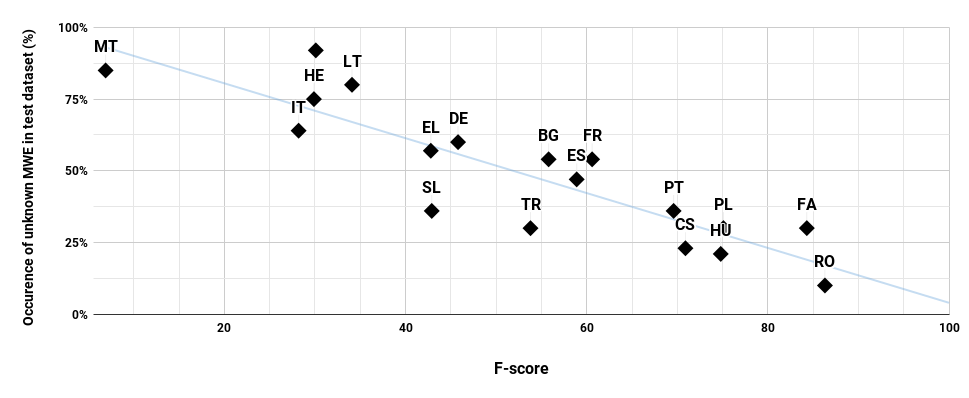
\includegraphics[height=5cm,keepaspectratio]{figures/alsaied-graph1.png}
\caption{Correlation between the ATILF-LLF 2 identification results for each language (F-score, on the x axis) and the percentage of \textbf{occurrences of test VMWEs unknown in the train set} (y axis).}
\label{fig:correlation}
\end{figure}
% ***********************************
%			Figure
% ***********************************
\begin{figure}
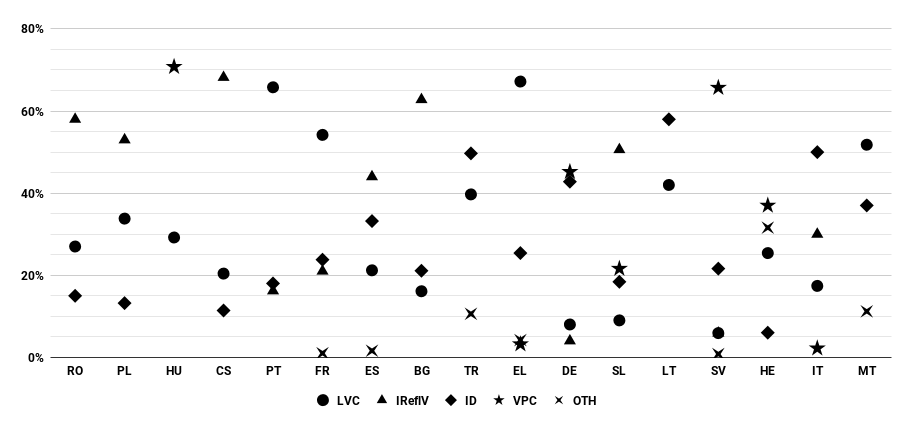
\includegraphics[width=\linewidth]{figures/alsaied-cats.png}
\caption{A graph ranking all languages except Farsi according to their F-scores. In each bar, the proportions of VMWE categories in the test set are shown using symbols.}
\label{fig:cats}
\end{figure}
% ***********************************
%			Related Work
% ***********************************
\section{Related work}
A popular VMWE identification\is{verbal multiword expression!identification} method is to use a sequence labeling approach, with IOB-based tagsets. For instance, \citet{diab-bhutada:2009:MWE09} apply a sequential SVM\is{support vector machine} to identify verb-noun\is{verbal multiword expression!verb-noun} idiomatic combinations in \ili{English}. Note also that three (out of seven) systems participating in the PARSEME shared task used such approach \citep{borocs2017,maldonado2017,W17-1707}.
Such an approach was also investigated for MWE identification in general (including verbal expressions) ranging from continuous expressions \citep{blunsom-baldwin:2006:EMNLP} to gappy ones \citep{Schneider14b}. Recently, neural networks have been successfully integrated into this framework \citep{legrand2016phrase,W17-1707}. 

VMWE identification can naturally take advantage of previously predicted syntactic parses. Some systems use them as soft constraints. For instance, the sequence labeling systems of the shared task and our system use them as source of features in their statistical tagging models. There also exist approaches using syntactic parses as hard constraints. For example, \citet{Baptista:2015} apply hand-crafted identification rules on them.  \citet{fazly-cook-stevenson:2009:CL} and \citet{nagyt-vincze:2014:MWE} propose a two-pass identification process consisting of candidate extraction followed by binary \isi{classification}. In particular, candidate extraction takes advantage of predicted syntactic parses, through the use of linguistic patterns. 

A joint syntactic analysis and VMWE identification approach using off-the-shelf parsers is another interesting alternative that has shown to help VMWE identification such as light-verb constructions \citep{Eryigit:2011:MES:2206359.2206365,Vincze:2010}. Some parsers integrate mechanisms into the parsing algorithm to identify MWEs on top of predicting the syntactic structure, like in \citet{Wehrli:2010} and \citet{constant-nivre:acl:2016}, our system being a simplified version of the latter.
% ***********************************
%			Conclusion and future work
% ***********************************
\section{Conclusion and future work}
This article presents a simple transition-based system devoted to VMWE identification and categorization. In particular, it offers a simple mechanism to handle discontinuity and embedding, which is a crucial point for VMWEs.
Results on the PARSEME Shared Task datasets show that our system is quite robust across languages, and achieves very competitive results. Its linear time complexity is also an asset.

\newpage
As future work, we would like to apply more sophisticated syntax-based features, as well as more advanced machine-learning techniques like neural networks. We also plan to investigate the use of a dynamic oracle \citep{goldberg:2012}.
% ***********************************
%			Acknowledgements
% ***********************************
\section*{Acknowledgements}
This work was partially funded by the French National Research Agency\\ (PARSEME-FR ANR-14-CERA-0001).

\section*{Abbreviations}

\begin{tabularx}{.49\textwidth}{ll}
\textsc{id} & Idiom\\ 
\textsc{iob}& inside outside beginning\\ 
\textsc{IReflV} & inherently reflexive verb  \\
\textsc{lvc} & light-verb construction  \\
\textsc{mwe} & multiword expression  \\
\end{tabularx}
\begin{tabularx}{.49\textwidth}{ll}
\textsc{mwt} & multiword token  \\
\textsc{oth} & other verbal MWE \\
\textsc{vmwe} & verbal multiword expression \\
\textsc{vpc} & verb-particle construction  \\ 
\\
\end{tabularx}
\largerpage
 
{\sloppy
\printbibliography[heading=subbibliography,notkeyword=this]
}
\end{document}
